%-*- program: xelatex -*-        
%-*- program: biber -*-`        
%-*- program: xelatex -*-
\documentclass[11pt]{article}
\usepackage[margin=0.75in]{geometry}            % See geometry.pdf to learn the layout options. There are lots.
\geometry{letterpaper}  
\usepackage{amsmath,textcomp,amssymb,geometry,graphicx,enumerate,upquote,color}
\usepackage{hyperref}
\usepackage{breqn}
\usepackage{float}
\usepackage{tikz}
\usepackage{array}
\usepackage{float}
\usepackage{amsfonts}
\def\Session{Fall 2015}
\usepackage[english]{babel}
\title{Drawdown Project - Simulation}
\author{Boying Gong, Xinyue Zhou}
\newenvironment{qparts}{\begin{enumerate}[{(}a{)}]}{\end{enumerate}}
\def\endproofmark{$\Box$}
\newenvironment{proof}{\par{\bf Proof}:}{\endproofmark\smallskip}
\begin{document}
\maketitle

\tableofcontents

\clearpage

%%%%%%%%%%%%
\section{AR(1)} %%%%
%%%%%%%%%%%%

We started from the simplest model AR(1):

\begin{equation}
X_t = \kappa_1X_{t-1} + \epsilon_t
\end{equation}

We simulate AR(1) for various values of the autoregressive parameter for $\kappa_1 \in (-1, 1)$ . Figure \ref{fig:AR1_risk_measures} shows the relationship between AR(1) coefficient and risk measures of interest including ES, VaR, volatility and CED. Note that for AR(1) model, the order one serial correlation is the the value of autoregressive parameter.

CED shows a decreasing trend when $\kappa_1\in(-1, -0.75)$ and an increasing trend when $\kappa_1 \in(-0.75, 1)$. As shown in Figure \ref{fig:AR1_risk_measures}, it becomes feasible for us to distinguish negative and positive serial correlation using the CED values. However, the other 3 risk measures are all symmetric about $\kappa_1 = 0$, and they increase as the absolute values of $\kappa_1$ increases.

For VaR, ES and CED, the derivative of risk measure values to $\kappa_1$ approaches to zero as  $\kappa_1$ goes to 0 and increase as $\kappa_1$ increase. The trend of derivatives reverse for CED. While the change of $\kappa_1$ has a comparatively larger influence around 0, the influence becomes weaker as we move to larger  $\kappa_1$ values.

\begin{figure}[H]
\centering
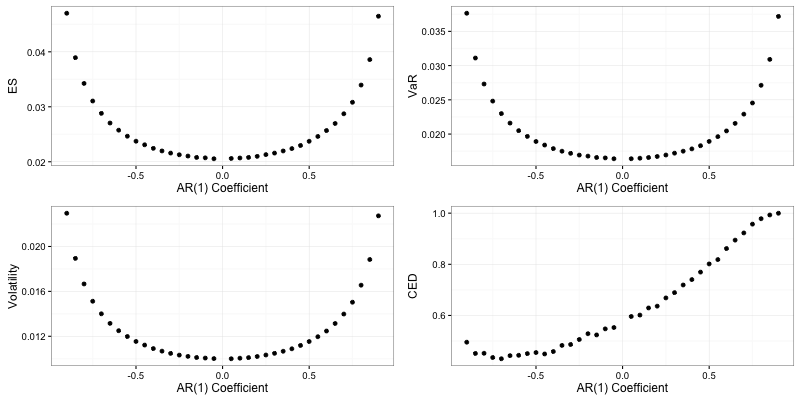
\includegraphics[width = 0.8\textwidth]{../figures/simulation/AR1_risk_measures}
\caption{AR(1): Relationship between auto-correlation coefficients and risk measures}
(Simulation path length: 1000, $\epsilon_t \sim N(0, 0.0001)$)
\label{fig:AR1_risk_measures}
\end{figure}

\begin{figure}[H]
\centering
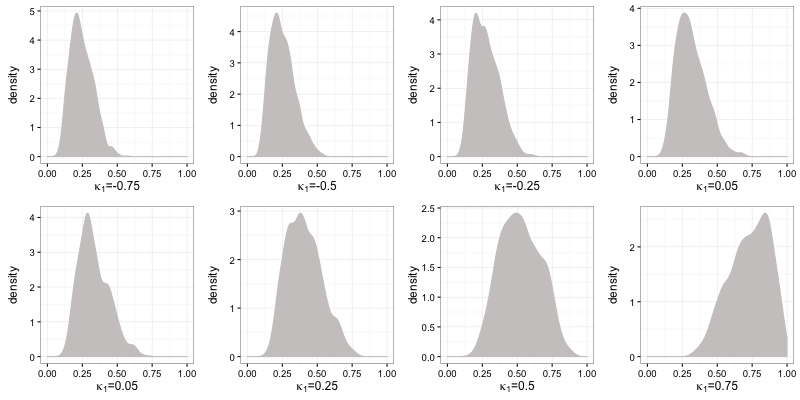
\includegraphics[width = 0.8\textwidth]{../figures/simulation/AR1_maxDrawdown_dist}
\caption{AR(1): Maximum drawdown distribution for various $\kappa_1$ values }
(Empirical distribution, path length = 1000, sample size = 1000, $\epsilon_t \sim N(0, 0.0001)$ )
\label{fig:AR1_maxDrawdown_dist}
\end{figure}

%%%%%%%%%%%%
\section{AR(2)} %%%%
%%%%%%%%%%%%

We then move to model AR(2):

\begin{equation}
X_t = \kappa_1X_{t-1} + \kappa_2X_{t-2}  + \epsilon_t
\end{equation}

Figure \ref{fig:AR2_risk_measures_pos} and \ref{fig:AR2_risk_measures_neg} shows the relationship between order one serial correlation and various risk measures.

\begin{figure}[H]
\centering
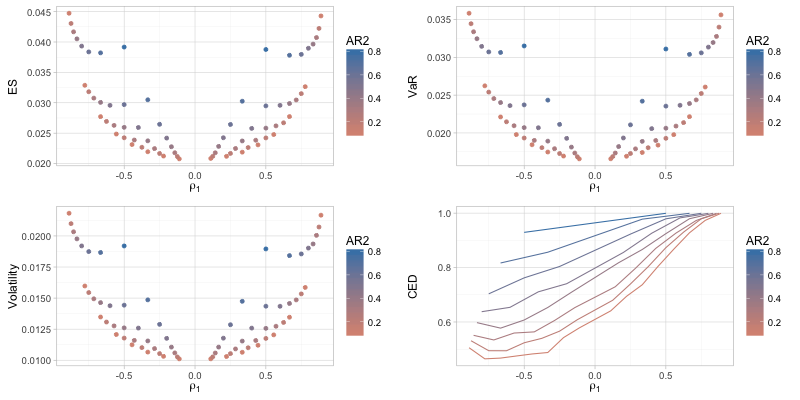
\includegraphics[width = 0.8\textwidth]{../figures/simulation/AR2_risk_measures_pos}
\caption{AR(2): Relationship between serial correlation $\rho_1$ and risk measures ($\kappa_2 > 0$)}
(Simulation path length: 1000, $\epsilon_t \sim N(0, 0.0001)$)
\label{fig:AR2_risk_measures_pos}
\end{figure}

\begin{figure}[H]
\centering
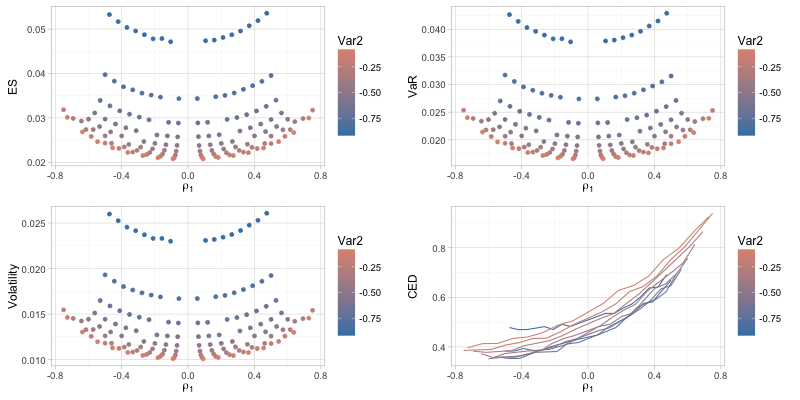
\includegraphics[width = 0.8\textwidth]{../figures/simulation/AR2_risk_measures_neg}
\caption{AR(2): Relationship between serial correlation $\rho_1$ and risk measures ($\kappa_2 < 0$)}
(Simulation path length: 1000, $\epsilon_t \sim N(0, 0.0001)$)
\label{fig:AR2_risk_measures_neg}
\end{figure}

\begin{figure}[H]
\centering
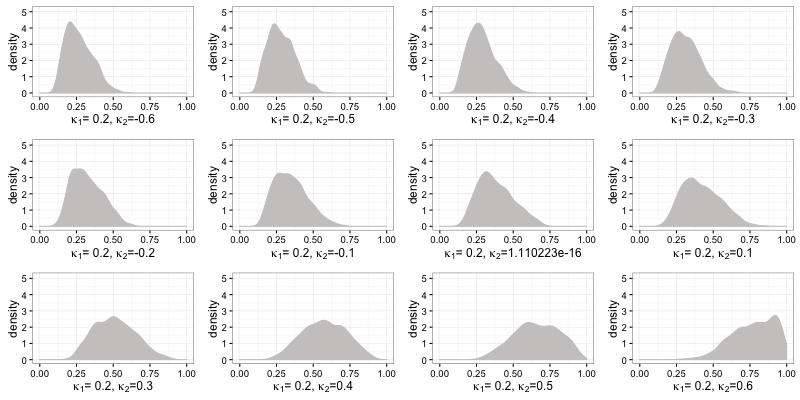
\includegraphics[width = 0.8\textwidth]{../figures/simulation/AR2_maxDrawdown_dist_kappa1_02}
\caption{AR(2): Maximum drawdown distribution for $\kappa_1 = 0.2$}
(Empirical distribution, path length = 1000, sample size = 1000, $\epsilon_t \sim N(0, 0.0001)$ )
\label{fig:AR2_maxDrawdown_dist_kappa1_02}
\end{figure}

\begin{figure}[H]
\centering
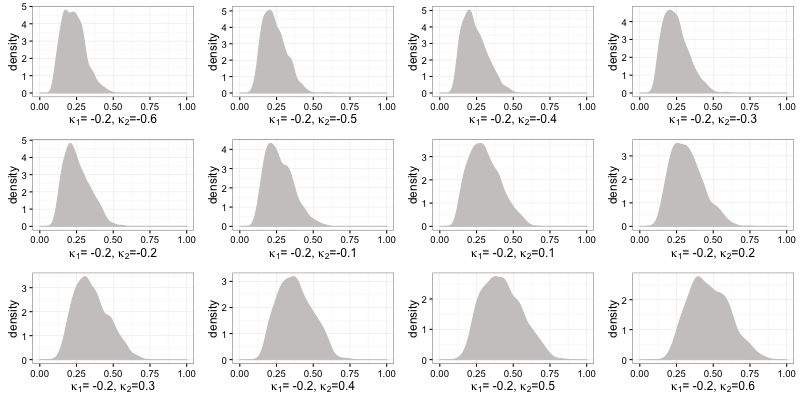
\includegraphics[width = 0.8\textwidth]{../figures/simulation/AR2_maxDrawdown_dist_kappa1_-02}
\caption{AR(2): Maximum drawdown distribution for $\kappa_1 = -0.2$}
(Empirical distribution, path length = 1000, sample size = 1000, $\epsilon_t \sim N(0, 0.0001)$ )
\label{fig:AR2_maxDrawdown_dist_kappa1_-02}
\end{figure}

%%%%%%%%%%%%
\section{MA(1)} %%%%
%%%%%%%%%%%%

\begin{figure}[H]
\centering
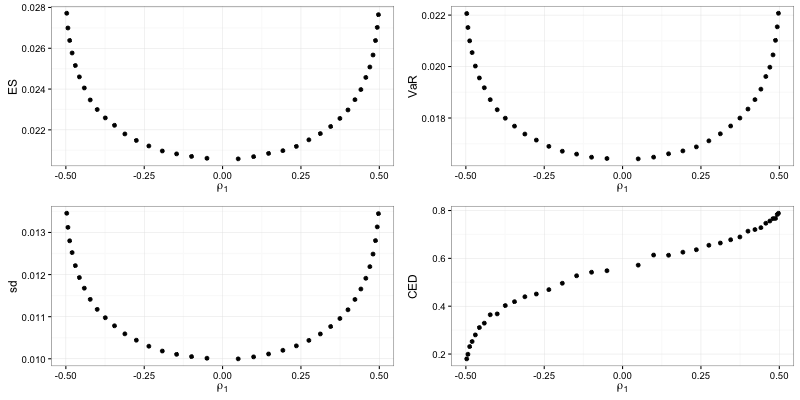
\includegraphics[width = 0.8\textwidth]{../figures/simulation/MA1_risk_measures_acf1}
\caption{MA(1): Relationship between serial correlation $\rho_1$ and risk measures}
(Simulation path length: 1000, $\epsilon_t \sim N(0, 0.0001)$)
\label{fig:MA1_risk_measures_acf1}
\end{figure}

\begin{figure}[H]
\centering
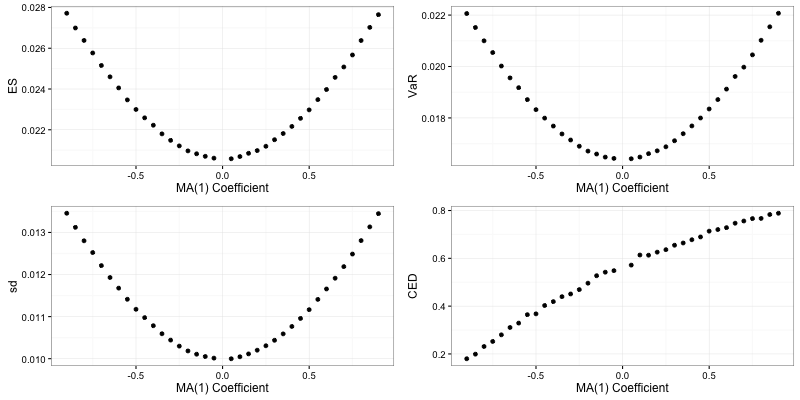
\includegraphics[width = 0.8\textwidth]{../figures/simulation/MA1_risk_measures_coefficient}
\caption{MA(1): Relationship between model coefficient and risk measures}
(Simulation path length: 1000, $\epsilon_t \sim N(0, 0.0001)$)
\label{fig:MA1_risk_measures_coefficient}
\end{figure}

\begin{figure}[H]
\centering
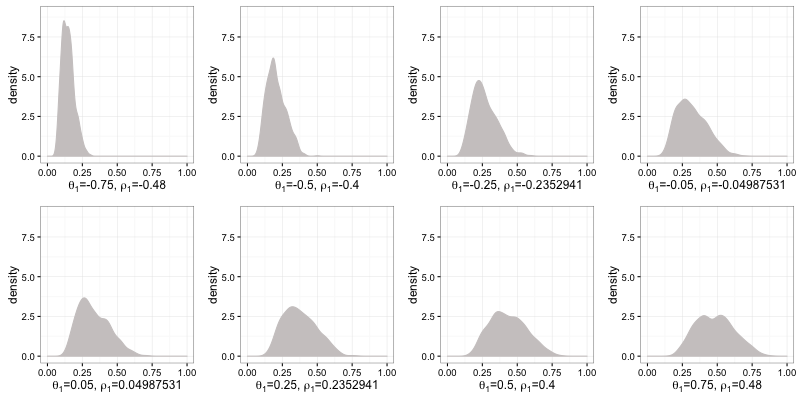
\includegraphics[width = 0.8\textwidth]{../figures/simulation/MA1_maxDrawdown_dist}
\caption{MA(1): Maximum drawdown distribution for various $\theta_1$ values}
(Empirical distribution, path length = 1000, sample size = 1000, $\epsilon_t \sim N(0, 0.0001)$ )
\label{fig:MA1_maxDrawdown_dist}
\end{figure}



%%%%%%%%%%%%
\section{MA(2)} %%%%
%%%%%%%%%%%%



%%%%%%%%%%%%%%%
\section{ARMA(1, 1)} %%%%
%%%%%%%%%%%%%%%




\end{document}
